\documentclass{article}

\usepackage{graphicx}
\usepackage{tikz}
\usepackage{tikzsymbols}
\usetikzlibrary{calc,patterns,shapes.geometric}
\pagestyle{empty}
\usepackage[margin=0pt]{geometry}
\geometry{papersize={14in,12in}}

\def\centerarc[#1](#2)(#3:#4:#5){\draw[#1] ($(#2)+({#5*cos(#3)},{#5*sin(#3)})$) arc (#3:#4:#5);}

\begin{document}
	\begin{figure}
		\centering
		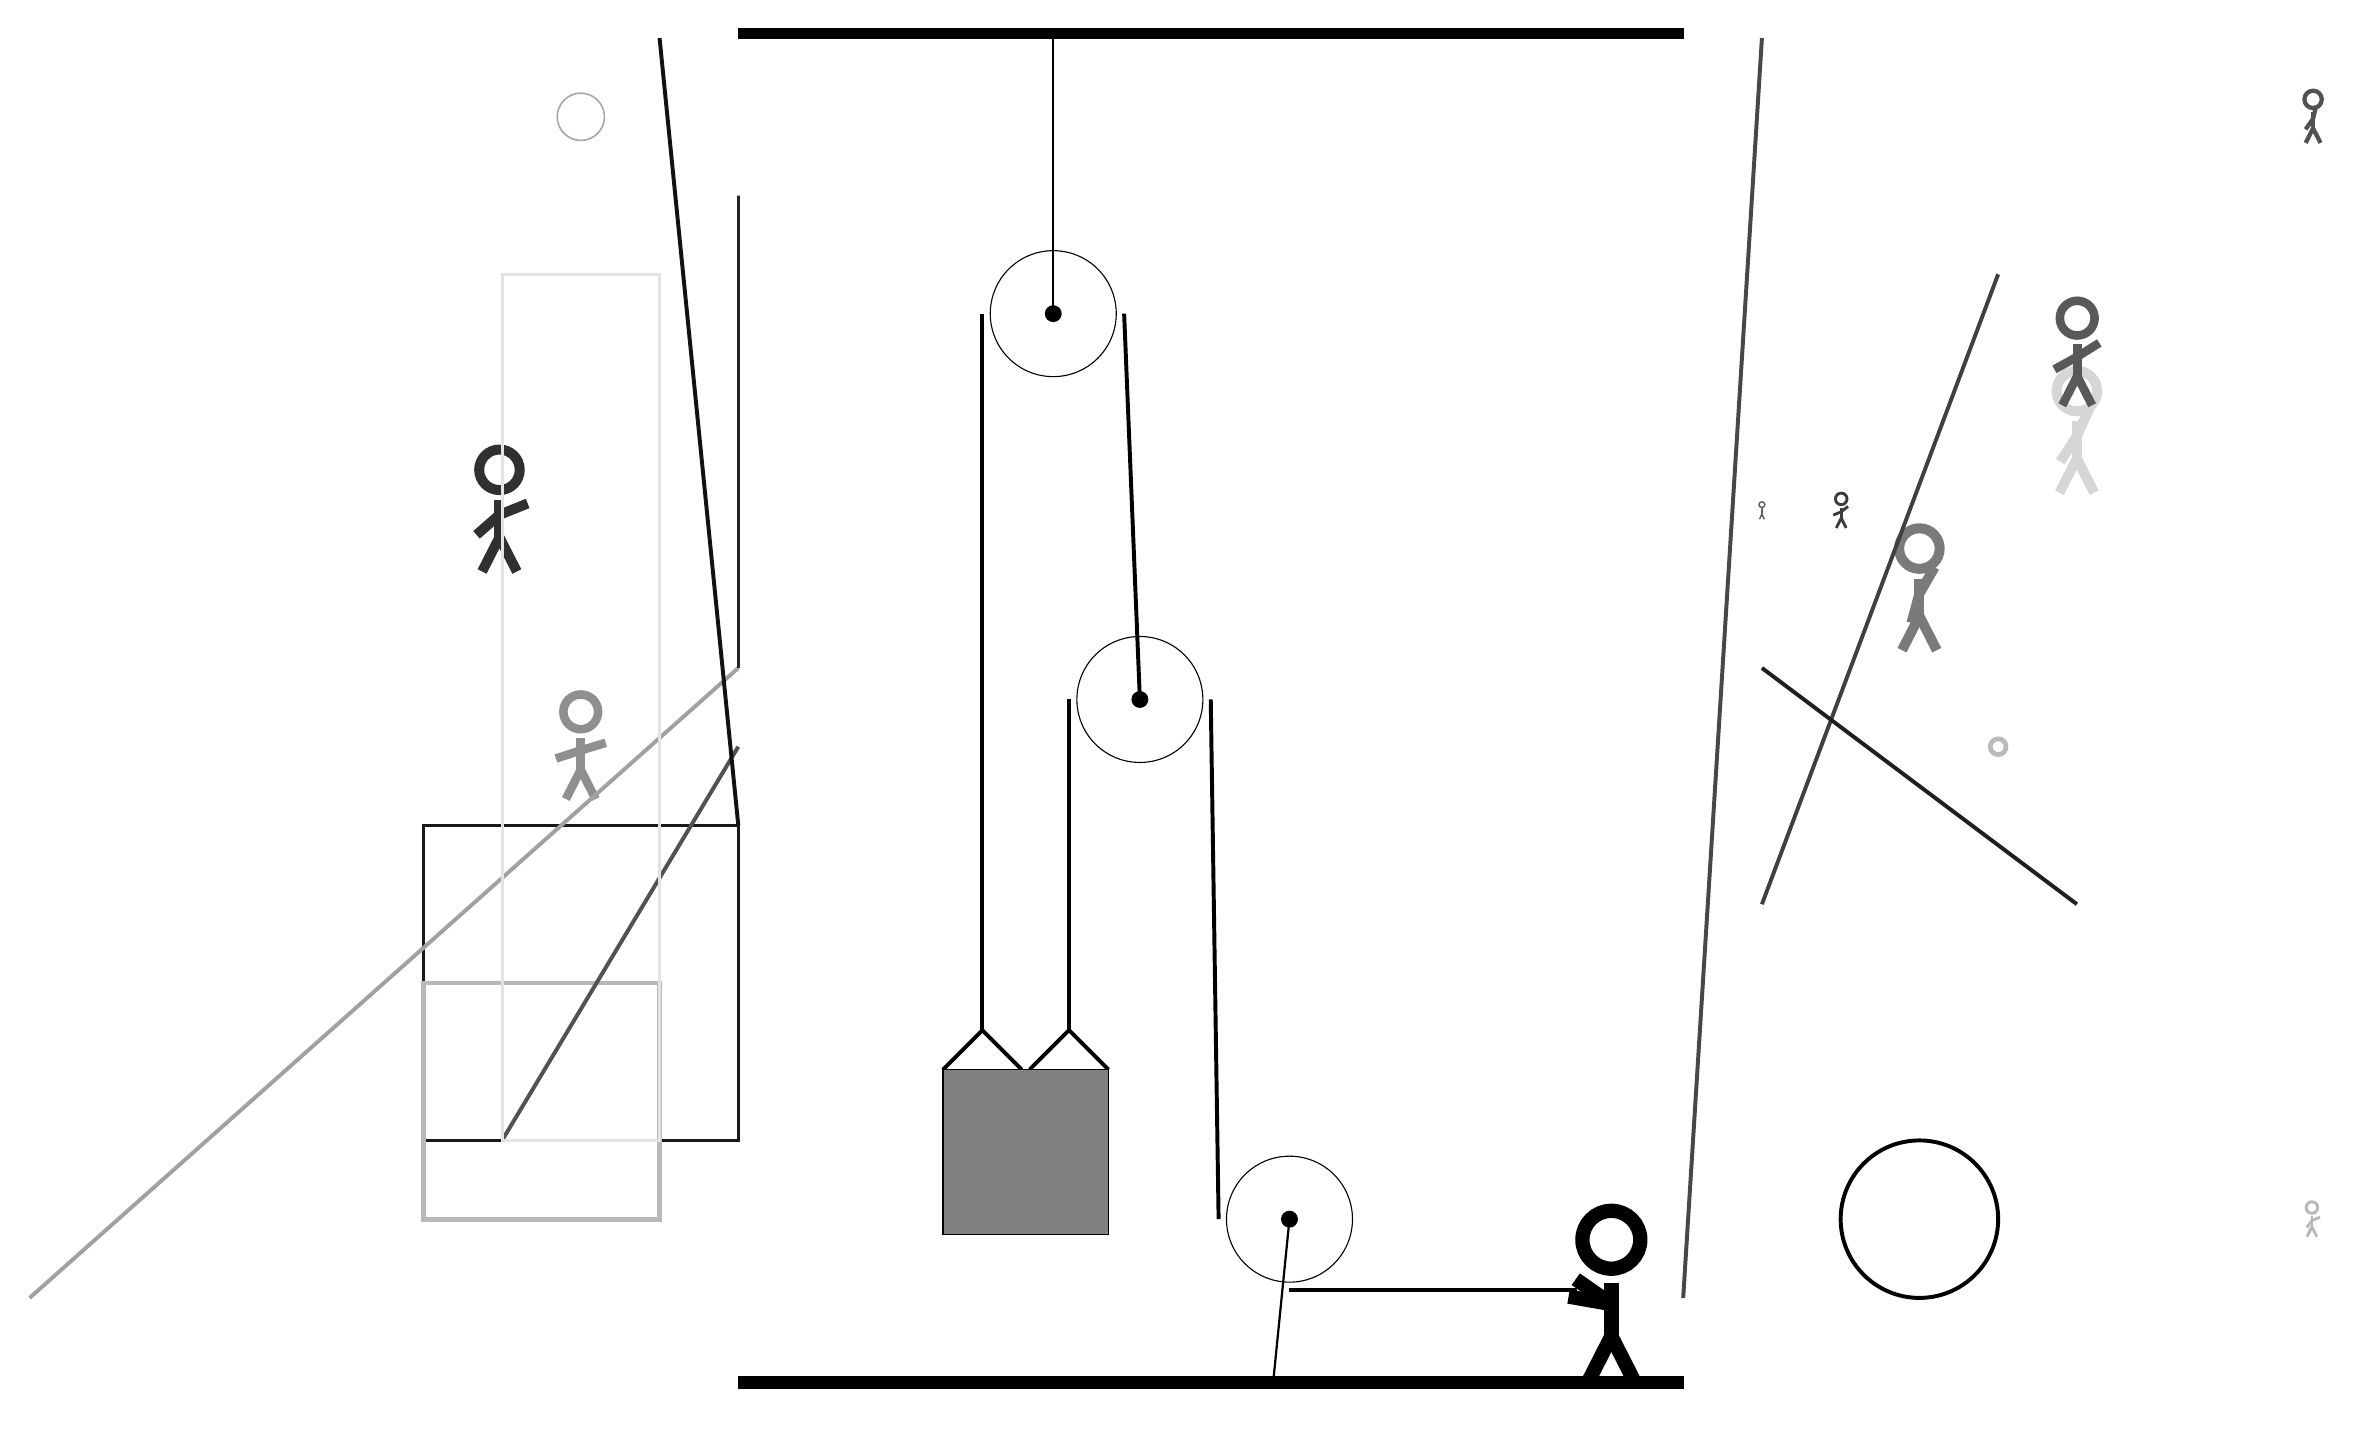
\begin{tikzpicture}
			%%%%% START %%%%%
			
			\draw[fill=black] (-2, 14) rectangle (10, 14.125);
			
			\draw (2, 10.5) circle (0.8);
			\draw[fill=black] (2, 10.5) circle (0.1);
			\draw[thick] (2, 10.5) -- (2, 14);
			
			\draw (3.1, 5.6) circle (0.8);
			\draw[fill=black] (3.1, 5.6) circle (0.1);
			
			\draw (5, -1) circle (0.8);
			\draw[fill=black] (5, -1) circle (0.1);
			\draw[thick] (5, -1) -- (4.8, -3);
			
			\draw[line width = 0.5mm]  (0.6, 0.9) -- (1.1, 1.4) -- (1.6, 0.9);
			\draw[line width = 0.5mm]  (1.7, 0.9) -- (2.2, 1.4) -- (2.7, 0.9);
			\draw[fill=black!50] (0.6, 0.9) rectangle (2.7, -1.2);
			
			\draw[line width = 0.5mm] (1.1, 10.5) -- (1.1, 1.4);
			\centerarc[line width = 0.5mm](2, 10.5)(0:180:0.9);
			\draw[line width = 0.5mm] (2.9, 10.5) -- (3.1, 5.6);
			\draw[line width = 0.5mm] (2.2, 5.6) -- (2.2, 1.4);
			\centerarc[line width = 0.5mm](3.1, 5.6)(0:180:0.9);
			\draw[line width = 0.5mm] (4.0, 5.6) -- (4.1, -1);
			\centerarc[line width = 0.5mm](5, -1)(180:270:0.9);
			\draw[line width = 0.5mm] (5, -1.9) -- (8.65, -1.9);
			
			\node[line width=0.2mm, color=black!44] at (-4, 5) {\Strichmaxerl[6][18][17]};
			
			\draw[line width=0.4mm, color=black!90] (-2, 0) rectangle (-6, 4);
			\node[line width=0.4mm, color=black!52] at (13, 7) {\Strichmaxerl[7][75][60]};
			\draw[line width=0.5mm, color=black!75](11, 3) -- (14, 11);
			
			\draw[line width=0.6mm, color=black!28] (-3, 2) rectangle (-6, -1);
			\draw [line width=0.2mm, color=black!35](-4, 13) circle (0.3);
			\node[line width=0.3mm, color=black!81] at (-5, 8) {\Strichmaxerl[7][41][22]};
			
			\node[line width=0.5mm, color=black!68] at (18, 13) {\Strichmaxerl[3][55][77]};
			\draw[line width=0.5mm, color=black!37](-2, 6) -- (-11, -2);
			\draw[line width=0.5mm, color=black!68](-5, 0) -- (-2, 5);
			\node[line width=0.4mm, color=black!28] at (18, -1) {\Strichmaxerl[2][55][21]};
			
			\draw [line width=0.6mm, color=black!27](14, 5) circle (0.1);
			\draw[line width=0.5mm, color=black!88](15, 3) -- (11, 6);
			\draw[line width=0.4mm, color=black!86] (-2, 6) rectangle (-2, 12);
			\node[line width=0.2mm, color=black!16] at (15, 9) {\Strichmaxerl[7][57][66]};
			\draw [line width=0.5mm, color=black!100](13, -1) circle (1.0);
			\node[line width=0.2mm, color=black!64] at (11, 8) {\Strichmaxerl[1][85][85]};
			
			\draw[line width=0.4mm, color=black!11] (-3, 0) rectangle (-5, 11);
			\draw[line width=0.5mm, color=black!93](-3, 14) -- (-2, 4);
			\node[line width=0.5mm, color=black!77] at (12, 8) {\Strichmaxerl[2][23][38]};
			\draw[line width=0.5mm, color=black!72](10, -2) -- (11, 14);
			\node[line width=0.2mm, color=black!65] at (15, 10) {\Strichmaxerl[6][29][32]};
			
			
			\node at (9, -2) {\Strichmaxerl[10][-35][170]};
			
			\draw[fill=black] (-2, -3) rectangle (10, -3.15);
			
			%%%%% END %%%%%
		\end{tikzpicture}
	\end{figure}	
\end{document}